%%%%%%%%%%%%%%%%%%%%%%%%%%%%%%%%%%%%%%%%%
% Beamer Presentation
% LaTeX Template
% Version 1.0 (10/11/12)
%
% This template has been downloaded from:
% http://www.LaTeXTemplates.com
%
% License:
% CC BY-NC-SA 3.0 (http://creativecommons.org/licenses/by-nc-sa/3.0/)
%
%%%%%%%%%%%%%%%%%%%%%%%%%%%%%%%%%%%%%%%%%

%----------------------------------------------------------------------------------------
%	PACKAGES AND THEMES
%----------------------------------------------------------------------------------------

\documentclass[14pt,handout]{beamer}
%%\documentclass[14pt]{beamer}

\mode<presentation> {

% The Beamer class slide themes
\usetheme{Madrid} %i was using this one

% Beamer class color themes

%\usecolortheme{albatross}

%\setbeamertemplate{footline} % To remove the footer line in all slides uncomment this line
%\setbeamertemplate{footline}[page number] % To replace the footer line in all slides with a simple slide count uncomment this line

%\setbeamertemplate{navigation symbols}{} % To remove the navigation symbols from the bottom of all slides uncomment this line
}

\usepackage{graphicx} % Allows including images
\usepackage{booktabs} % Allows the use of \toprule, \midrule and \bottomrule in tables
\usepackage{hyperref}
\usepackage{helvet}
\usepackage[T1]{fontenc}
\usepackage{textcomp}

%----------------------------------------------------------------------------------------
%	TITLE PAGE
%----------------------------------------------------------------------------------------

\title[Genome Assembly]{Problems in Genome Assembly} % The short title appears at the bottom of every slide, the full title is only on the title page

\author{C. Ryan Campbell} % Your name
\institute[Duke] % Your institution as it will appear on the bottom of every slide, may be shorthand to save space
{
Duke University \\ % Your institution for the title page
\medskip
\textit{c.ryan.campbell@duke.edu} % Your email address
}
\date{24 Oct 2017} % Date, can be changed to a custom date

\begin{document}

\begin{frame}
\titlepage % Print the title page as the first slide
\end{frame}

\begin{frame}
\frametitle{Overview} % Table of contents slide, comment this block out to remove it
\tableofcontents % Throughout your presentation, if you choose to use \section{} and \subsection{} commands, these will automatically be printed on this slide as an overview of your presentation
\end{frame}

%----------------------------------------------------------------------------------------
%	PRESENTATION SLIDES
%----------------------------------------------------------------------------------------

%------------------------------------------------
\begin{frame}
\frametitle{Today's Goals}
\begin{itemize}
	\item<+-> Why is assembly important?
	\item<+-> What are the differences in long and short read platforms?
	\item<+-> How do these differences impact assembly?
\end{itemize}
\end{frame}

%------------------------------------------------
\section{Genome Assembly}
%------------------------------------------------

%------------------------------------------------
\begin{frame}
\frametitle{Genome Assembly}
\begin{itemize}
	\item<+-> Mapping (or assembling) all the bases in the genome of an organism
	\item<+-> List all the bases for each chromosome
	\item<+-> Annotate the genes and exonic/intronic regions
	\item<+-> Why do we want to do this?
	\item<+-> Is this assembly for an individual or a species?
\end{itemize}
\end{frame}

%------------------------------------------------
\subsection{The Old Way}
%------------------------------------------------

%------------------------------------------------
\begin{frame}
\frametitle{Assembling the Human Genome}
\begin{itemize}
	\item<+-> Was once limited by the throughput of Sanger sequencing
	\item<+-> Genomic DNA was separated by chromosome
	\item<+-> Cloned into bacteria
	\item<+-> Sequenced little by little
\end{itemize}
\end{frame}

%------------------------------------------------
\begin{frame}
\frametitle{Shotgun Sequencing}
\begin{itemize}
	\item<+-> Eventually we moved on to ``shotgun'' sequencing
	\item<+-> Randomly sequence as much of the genome as possible
	\item<+-> Assemble into a complete genome
	\item<+-> What are the possible issues with this method?
\end{itemize}
\end{frame}

%------------------------------------------------
\subsection{The New Way}
%------------------------------------------------

%------------------------------------------------
\begin{frame}
\frametitle{Next Generation Sequencing (NGS)}
\begin{itemize}
	\item<+-> Still technically a ``shotgun'' method
	\item<+-> NGS produces a lot more data than Sanger
	\item<+-> Think of it as many shotguns
	\item<+-> What are the types of NGS we've talked about?
\end{itemize}
\end{frame}

%------------------------------------------------
\begin{frame}
\frametitle{Illumina - Short Reads}
\begin{itemize}
	\item<+-> ``Short'' reads - 100-250 bp
	\item<+-> Sequence as a paired-end read
	\item<+-> Can cover up to 500bp of an 800bp fragment
	\item<+-> Accurate and cheap
\end{itemize}
\end{frame}

%------------------------------------------------
\begin{frame}
\frametitle{PacBio - Long Reads}
\begin{itemize}
	\item<+-> ``Long'' read - greater than 1,000 bp
	\item<+-> Sequence fragment in a loop (shorter fragments get sequenced at higher coverage)
	\item<+-> High end now up to 20,000 bp
	\item<+-> Less accurate, more expensive per base
\end{itemize}
\end{frame}

%------------------------------------------------
\section{What is the best approach?}
%------------------------------------------------

%------------------------------------------------
\begin{frame}
\frametitle{What is the best approach?}
\begin{itemize}
	\item<+-> Given a finite budget should you:
	\begin{itemize}
		\item<+-> Use a lot of ``short'' reads?
		\item<+-> Use fewer ``long'' reads?
		\item<+-> Use even less of a mix of both?
	\end{itemize}
\end{itemize}
\end{frame}

%------------------------------------------------
\section{Assessing Genome Quality}
%------------------------------------------------

%------------------------------------------------
\begin{frame}
\frametitle{How do we know what is ``best''}
\begin{itemize}
	\item<+-> How is genome assembly quality measured?
	\item<+-> What makes a ``good'' genome?
\end{itemize}
\end{frame}

%------------------------------------------------
\begin{frame}
\frametitle{How do we know what is ``best''}
\end{frame}

%------------------------------------------------
\begin{frame}
\frametitle{How do we know what is ``best''}
\begin{itemize}
	\item<+-> Quantitatively (N50 scores)
	\begin{itemize}
		\item<+-> How much of the expected genome have you assembled?
		\item<+-> How long are the pieces of the genome you have assembled?
	\end{itemize}
	\item<+-> Qualitatively (BUSCO)
	\begin{itemize}
		\item<+-> Are the genomic features we expect to be there present?
		\item<+-> Look for commonly conserved genes
		\item<+-> Benchmarking Universal Single-Copy Orthologs
	\end{itemize}
\end{itemize}
\end{frame}

%------------------------------------------------
\begin{frame}
\frametitle{Common Terms}
\begin{itemize}
	\item<+-> Contig
	\begin{itemize}
		\item<+-> A run of \underline{contig}uous bases
		\item<+-> No gaps allowed
	\end{itemize}
	\item<+-> Scaffold
	\begin{itemize}
		\item<+-> A set of contigs \underline{scaffold}ed together with gaps of N's
		\item<+-> Must know how far apart the contigs are
	\end{itemize}
\end{itemize}
\end{frame}

%------------------------------------------------
\begin{frame}
\frametitle{Scaffold N50}
\begin{itemize}
	\item<+-> Measure of genome assembly quality
	\item<+-> Arrange the scaffolds from longest to shortest
	\item<+-> N50 = Length of the scaffold at 50\% of the total genome size
	\item<+-> What is a perfect N50?
\end{itemize}
\end{frame}

%WHAT IS N50
%------------------------------------------------
\begin{frame}
\frametitle{N50}
\begin{center}
	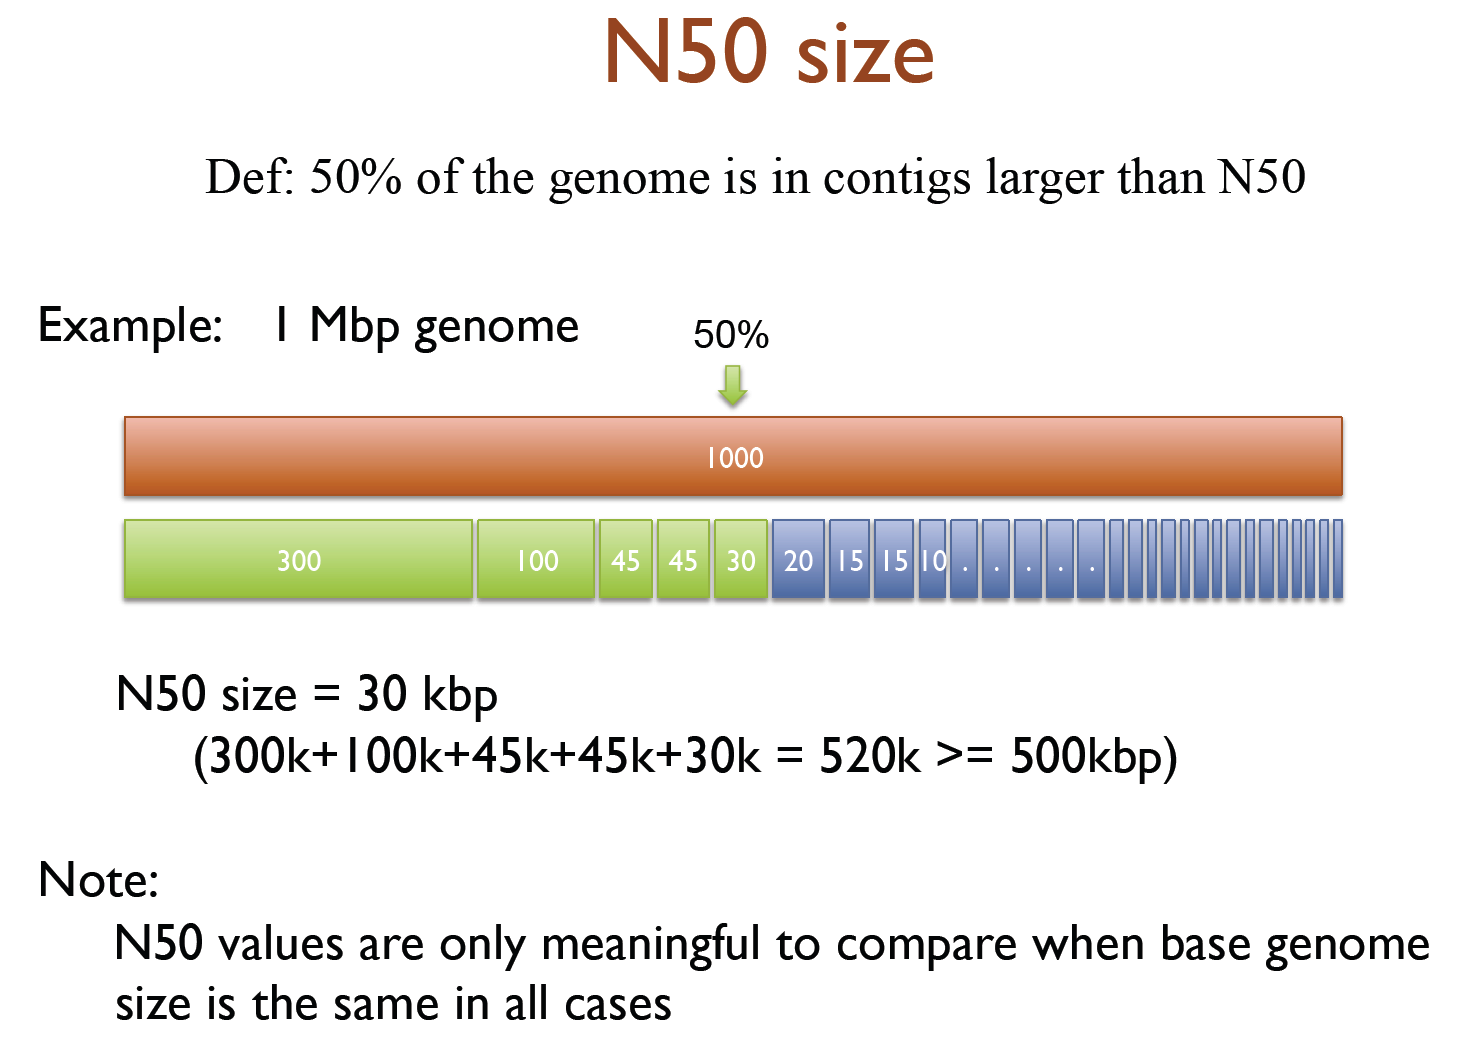
\includegraphics[width=1\textwidth]{images_20171024_n50.png}
\end{center}
\end{frame}


%------------------------------------------------
\subsection{Activity}
%------------------------------------------------
%check progress at 5 minute intervals (5, 10, 15-stop?)
%track N50 etc
%estimate "genome" size
%------------------------------------------------
\begin{frame}
\frametitle{The Problem}
\begin{itemize}
	\item<+-> Common Assembly Problems:
	\item<+-> Size - 3bil bp = 5,000 books
	\item<+-> Chromosomal Arrangement - not just ``base 1-3,000,000,000''
	\item<+-> Repeats - tricky regions that are common in mammals
\end{itemize}
\end{frame}

%------------------------------------------------
\begin{frame}
\frametitle{Your Directions}
\begin{itemize}
	\item<+-> Assemble the sequence data your group has been given
	\item<+-> Should make a coherent paragraph, taken from a speech
	\item<+-> The ``data'' are randomly generated reads:
	\item<+-> Long - 75 characters, error prone
	\item<+-> Short - 16 characters, accurate 
\end{itemize}
\end{frame}

%------------------------------------------------
\begin{frame}
\frametitle{Your ``Output''}
\begin{enumerate}
	\item<+-> Estimate paragraph length
	\item<+-> Estimate the number of repeats
	\item<+-> Estimate the proportion of errors
	\item<+-> Estimate your contig N50
\end{enumerate}
\begin{itemize}
	\item<+-> IMPORTANT: ``|'' character is the end of the read
	\item<+-> 15-20 mins
\end{itemize}
\end{frame}

\begin{frame}
\frametitle{The Answer}
\ttfamily
\small
Even though large tracts of Europe and many old and famous States have fallen or may fall into the grip of the Gestapo and all the odious apparatus of Nazi rule, we shall not flag or fail. We shall go on to the end. We shall fight in France, we shall fight on the seas and oceans, we shall fight with growing confidence and growing strength in the air, we shall defend our island, whatever the cost may be. We shall fight on the beaches, we shall fight on the landing grounds, we shall fight in the fields and in the streets, we shall fight in the hills; we shall never surrender.
\end{frame}

\begin{frame}
\frametitle{The Answer}
\ttfamily
\small
Even though large tracts of Europe and many old and famous States have fallen or may fall into the grip of the Gestapo and all the odious apparatus of Nazi rule\underline{, we shall} not flag or fail\underline{. We shall} go on to the end\underline{. We shall fight} in France\underline{, we shall} fight on the seas and oceans\underline{, we shall fight} with growing confidence and growing strength in the air\underline{, we shall} defend our island, whatever the cost may be\underline{. We shall fight} on the beaches\underline{, we shall fight} on the landing grounds\underline{, we shall fight} in the fields and in the streets\underline{, we shall fight} in the hills\underline{; we shall} never surrender.

\textit{470 chars, 581 w/spaces}
\textit{11 repeats}
\end{frame}


%------------------------------------------------
\section{The New(est) Way}
%------------------------------------------------

%------------------------------------------------
\begin{frame}
\frametitle{The New(est) Ways}
\begin{itemize}
	\item<+-> Bio-Nano
	\item<+-> 10X Genomics
	\item<+-> Hi-C 
\end{itemize}
\end{frame}

%------------------------------------------------
\subsection{BioNano}
%------------------------------------------------

%------------------------------------------------
\begin{frame}
\frametitle{BioNano Genomics}
\begin{itemize}
	\item<+-> Technology to ``super''-scaffold long stretches
	\item<+-> Prepare high quality DNA, keeping as much of the chomosome intact as possible
	\item<+-> Flourescence-tag sites with a known 8bp sequence
	\item<+-> Use this as a backbone to build longer scaffolds
\end{itemize}
\end{frame}

%------------------------------------------------
\begin{frame}
\frametitle{BioNano}
\begin{columns}
	\begin{column}{0.3\textwidth}
		\begin{itemize}
			\item<+-> Collect long DNA
			\item<+-> Label known 8bp sites
			\item<+-> Image
		\end{itemize}
		\end{column}
	\begin{column}{0.7\textwidth}
		\begin{center}
     		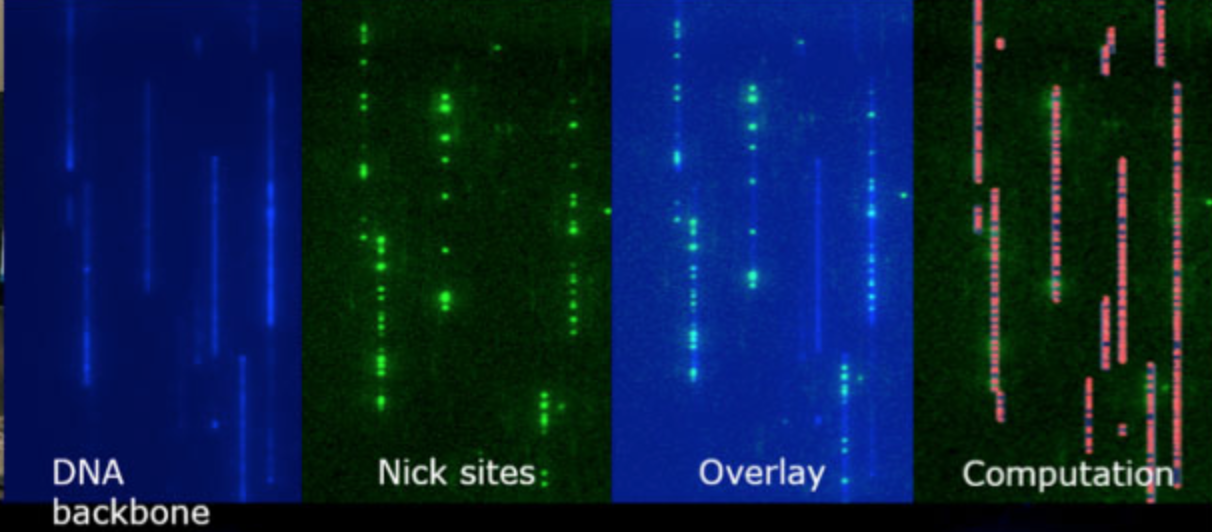
\includegraphics[width=1\textwidth]{images_20171024_bionano.png}
     	\end{center}
	\end{column}
\end{columns}
\end{frame}

%restriction site mapping across whole chromosomes
%carefully prep DNA w/o breaking up chromosomes
%image locations of restriction sites

%------------------------------------------------
\subsection{10X}
%------------------------------------------------

%------------------------------------------------
\begin{frame}
\frametitle{10X Genomics}
\begin{itemize}
	\item<+-> Built on Illumina technology
	\item<+-> Within oil droplets - barcode large DNA (100kb) and then fragment
	\item<+-> Sequence as usual
	\item<+-> Use the barcodes to successfully rebuild the 100kb pieces
	\item<+-> Simulates long read PacBio tech with Illumina
\end{itemize}
\end{frame}

%barcoding system for longer scaffolds
%oil-based, barcode everything across a ~100kb fragment with the same tag
%

%------------------------------------------------
\begin{frame}
\frametitle{10X Genomics}
\begin{columns}
	\begin{column}{0.4\textwidth}
		\begin{itemize}
			\item<+-> Label 100kb frags
			\item<+-> Barcode within beads
			\item<+-> Seq and reassemble
		\end{itemize}
		\end{column}
	\begin{column}{0.6\textwidth}
		\begin{center}
     		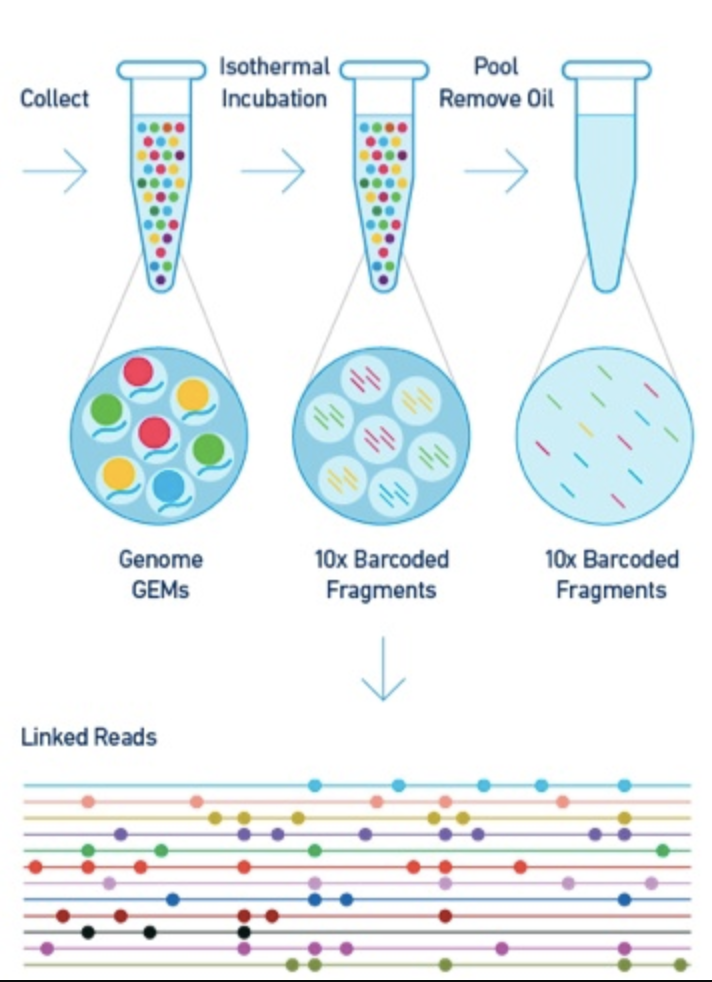
\includegraphics[width=1\textwidth]{images_20171024_10X.png}
     	\end{center}
	\end{column}
\end{columns}
\end{frame}



%------------------------------------------------
\subsection{Hi-C}
%------------------------------------------------

%------------------------------------------------
\begin{frame}
\frametitle{Hi-C}
\begin{itemize}
	\item<+-> Within a nucleus link DNA as it is found naturally
	\item<+-> Connects neighboring DNA sites, even across chromosomes
	\item<+-> Fragment and sequence, maintaining these linkages
	\item<+-> Captures a snapshot of chromosomal interactions
\end{itemize}
\end{frame}

%------------------------------------------------
\begin{frame}
\frametitle{Hi-C}
\begin{columns}
	\begin{column}{0.3\textwidth}
		\begin{itemize}
			\item<+-> Link nuclear DNA
			\item<+-> Fragment
			\item<+-> Sequence across linkage
		\end{itemize}
		\end{column}
	\begin{column}{0.7\textwidth}
		\begin{center}
     		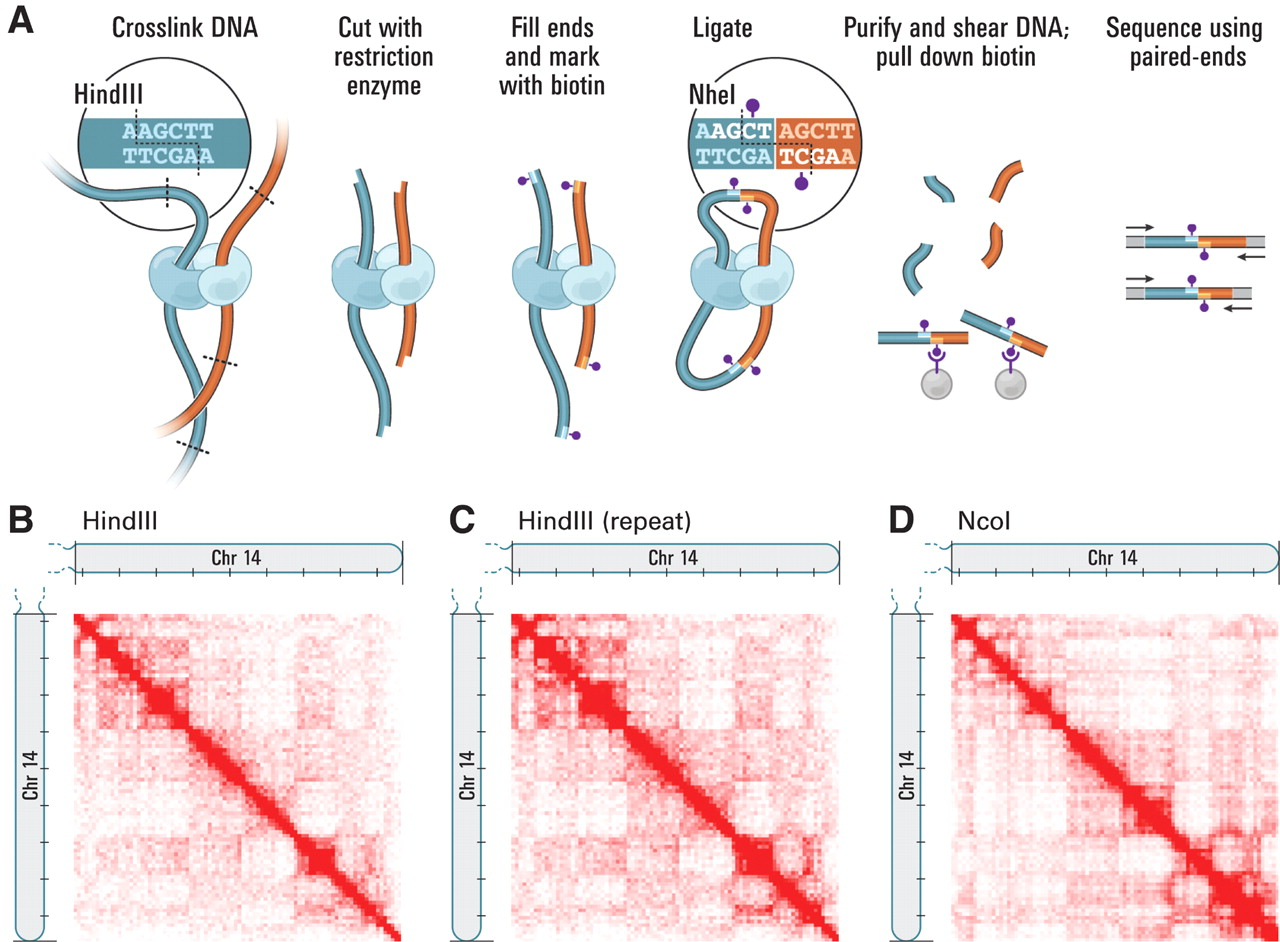
\includegraphics[width=1\textwidth]{images_20171024_hic.jpg}
     	\end{center}
	\end{column}
\end{columns}
\end{frame}





%------------------------------------------------
\begin{frame}
\frametitle{Hi-C}
\begin{itemize}
	\item<+-> Two main uses:
	\item<+-> 1) What parts of the genome are interacting with others?
	\begin{itemize}
		\item<+-> Open chromatin regions
		\item<+-> Interactions across chromosomes
	\end{itemize}
	\item<+-> 2) Which fragments are on the same chromosome?
	\begin{itemize}
		\item<+-> Much of the data is within chromosome
		\item<+-> Can use to improve assembly
	\end{itemize}
\end{itemize}
\end{frame}


%captures snapshot of chromosomal interactions
%form links across separate chromosomes based on nuclear location
%capture interactions
%
%how does this help assembly?

%------------------------------------------------
\section{What problems remain?}
%------------------------------------------------

%------------------------------------------------
\begin{frame}
\frametitle{Remaining Problems}
\begin{itemize}
	\item<+-> \underline{Centromeres} - very long and oddly repetitive
	\item<+-> \underline{Cost} - still expensive, especially to get structural variation
	\item<+-> \underline{Chasing down humans} - there are always techniques and features that are available to human biologists that other model organisms (and non-model organisms) are pursuing
\end{itemize}
\end{frame}

%centromeres


%------------------------------------------------
\begin{frame}
\Huge{\centerline{The End}}
\end{frame}

%----------------------------------------------------------------------------------------

\end{document} 